% ============================================================
%  Final Project Review -- Beamer slides (14 slides)
%  When Does Context Compression Break? A Robustness Study of ACON
%  Compile with: tectonic -X compile finalreview_slides.tex
%           or: pdflatex finalreview_slides.tex  (run twice)
% ============================================================
\documentclass[aspectratio=169,10pt]{beamer}

\usetheme{Madrid}
\usecolortheme{default}
\setbeamertemplate{navigation symbols}{}
\setbeamertemplate{frametitle continuation}{}
\setbeamertemplate{caption}[numbered]
\setbeamerfont{block title}{size=\normalsize}
\setbeamertemplate{itemize items}[circle]

\usepackage[T1]{fontenc}
\usepackage{lmodern}
\usepackage{amsmath,amssymb,mathtools}
\usepackage{booktabs}
\usepackage{graphicx}
\usepackage{tikz}
\usetikzlibrary{arrows.meta,positioning,calc,fit,shapes.geometric}
\usepackage{pgfplots}
\pgfplotsset{compat=1.16}

% tighter lists
\setlength{\leftmargini}{1.4em}
\setlength{\leftmarginii}{1.2em}

% shorthand colours used across the diagrams
\definecolor{envblue}{RGB}{31,80,140}
\definecolor{cmpgreen}{RGB}{28,110,60}
\definecolor{ctlorange}{RGB}{190,105,10}
\definecolor{metviolet}{RGB}{110,45,140}

\title[When Does Context Compression Break?]{When Does Context Compression Break?}
\subtitle{A Robustness Study of ACON for Long-Horizon LLM Agents}

\author[Ayush Rahate \& Rohit Chauhan]{
  \begin{tabular}{r@{\hspace{0.8em}}l}
    \textbf{123CS0006} & Ayush Rahate\\
    \textbf{123CS0054} & Rohit Chauhan
  \end{tabular}
}

\institute[IIITDM Kurnool]{
  Department of Computer Science and Engineering\\
  Indian Institute of Information Technology\\
  Design and Manufacturing, Kurnool
}

\date[Final Review]{Final Project Review \\ November 2026}

% ------------------------------------------------------------
\begin{document}

% ============================== 1. TITLE
{
\setbeamertemplate{footline}{}
\begin{frame}[plain]
  \vspace{-0.3cm}
  \begin{center}
    \includegraphics[height=1.25cm]{"png college logo".png}
  \end{center}
  \vspace{-0.55cm}
  {\setbeamerfont{title}{size=\large,series=\bfseries}%
   \setbeamerfont{subtitle}{size=\scriptsize}%
   \setbeamerfont{author}{size=\scriptsize}%
   \setbeamerfont{institute}{size=\tiny}%
   \setbeamerfont{date}{size=\tiny}%
   \titlepage}
  \vspace{-0.85cm}
  \begin{center}
    \scriptsize\textbf{Project Supervisor:} Dr.~N.~Srinivas Naik
  \end{center}
\end{frame}
}

% ============================== 2. PROBLEM STATEMENT
\section{Problem Statement}
\begin{frame}{Problem Statement}
\begin{block}{Problem}
\small
ACON~\cite{ACON} compresses an agent's history once it exceeds a token threshold
$T_{\mathrm{hist}}$. \textbf{How does task success depend on how often we
compress}, on \textbf{held-out} tasks, with \textbf{open-weight} models --- and
what breaks when it fails?
\end{block}
\vspace{-0.1cm}
\begin{columns}[T]
\begin{column}{0.47\textwidth}
\begin{alertblock}{Why it matters}
\footnotesize
\begin{itemize}
  \item ACON reports \textbf{one} threshold only; lowering $T_{\mathrm{hist}}$
        is the natural way to save more tokens
  \item ACON's combined history $+$ observation setting loses
        $I=\mathbf{-9.5}$ points~\cite{ACON} --- the motivation for our
        mid-semester proposal
\end{itemize}
\end{alertblock}
\begin{block}{Research questions}
\footnotesize
\begin{itemize}
  \item[\textbf{RQ1}] Does the combined-compression penalty reproduce?
  \item[\textbf{RQ2}] How does success depend on $T_{\mathrm{hist}}$?
  \item[\textbf{RQ3}] What causes the change, and can it be removed?
\end{itemize}
\end{block}
\end{column}
\begin{column}{0.51\textwidth}
\begin{block}{Formulation}
\footnotesize
Agent step (frozen $\theta$):\; $a_t = M(h'_{t-1},\,o'_t;\,\theta)$\\[3pt]
Trigger steps:\;
$\mathcal{K}(T_{\mathrm{hist}})=\{\,t : |h'_{t-1}\oplus(o'_t,a_t)|>T_{\mathrm{hist}}\,\}$
\[
h'_t=\begin{cases} f_h\big(h'_{t-1}\oplus(o'_t,a_t);\,g\big) & t\in\mathcal{K}\\
h'_{t-1}\oplus(o'_t,a_t) & \text{otherwise}\end{cases}
\]
Gain:\; $\Delta(\pi)=\mathbb{E}[R(\pi)]-\mathbb{E}[R(\pi_\varnothing)]$\\[2pt]
Cost:\; $C(\pi)=\sum_t\big(|h'_{t-1}|+|o'_t|\big)$\\[2pt]
Interaction:\; $I=\Delta(\pi_{ho})-\Delta(\pi_h)-\Delta(\pi_o)$\par\smallskip
\centering $R$: task success \quad $g$: guideline \quad lower $T_{\mathrm{hist}}$
$\Rightarrow$ more rewrites
\end{block}
\end{column}
\end{columns}
\end{frame}

% ============================== 3-4. LITERATURE
\section{Literature Review}
\begin{frame}{Literature Review (1/2): Existing Methods}
\begin{columns}[T]
\begin{column}{0.32\textwidth}
\begin{block}{ACON \cite{ACON}}
\footnotesize
\begin{itemize}
  \item LLM summarises history and observations past a token threshold
  \item Guideline optimised in natural language
  \item \textbf{Peak tokens $\downarrow$ 26--54\%}, accuracy kept
\end{itemize}
\end{block}
\end{column}
\begin{column}{0.32\textwidth}
\begin{block}{SAC \cite{SAC}}
\footnotesize
\begin{itemize}
  \item Anchor tokens absorb context via bidirectional attention
  \item Only anchor KV is kept
  \item \textbf{54.95 F1} at $15\times$ (EPL 51.52)
\end{itemize}
\end{block}
\end{column}
\begin{column}{0.32\textwidth}
\begin{block}{LLMLingua \cite{LLMLingua}}
\footnotesize
\begin{itemize}
  \item Drops low-information tokens using a small LM
  \item Task-agnostic, single-step
  \item Only \textbf{39.3\%} on AppWorld history
\end{itemize}
\end{block}
\end{column}
\end{columns}
\vspace{0.05cm}
\begin{columns}[T]
\begin{column}{0.32\textwidth}
\begin{block}{SWE-Pruner \cite{SWEPruner}}
\footnotesize
\begin{itemize}
  \item 0.6B line classifier guided by an agent-written goal hint
  \item \textbf{Tokens $\downarrow$ 23--38\%}
  \item Resolve rate $+$1.2--1.4 points
\end{itemize}
\end{block}
\end{column}
\begin{column}{0.32\textwidth}
\begin{block}{MEM1 / MemAgent \cite{MEM1,MemAgent}}
\footnotesize
\begin{itemize}
  \item Agent trained with RL to keep a bounded memory
  \item 8K window $\to$ 3.5M-token QA, $<$10\% loss
  \item \textcolor{red!70!black}{Needs agent weights}
\end{itemize}
\end{block}
\end{column}
\begin{column}{0.32\textwidth}
\begin{alertblock}{Takeaway}
\footnotesize
Each method is evaluated at \textbf{one} operating point, usually on the
split it was tuned on.\\[2pt]
\textbf{Open:} how robust is the benefit to \emph{compression frequency}, on
held-out tasks?
\end{alertblock}
\end{column}
\end{columns}
\end{frame}

\begin{frame}{Literature Review (2/2): Comparison}
\centering
\scriptsize
\renewcommand{\arraystretch}{1.2}
\setlength{\tabcolsep}{3.5pt}
\resizebox{\textwidth}{!}{%
\begin{tabular}{lcccccc}
\toprule
\textbf{Property} & \textbf{ACON}~\cite{ACON} & \textbf{SAC}~\cite{SAC} &
\textbf{SWE-Pruner}~\cite{SWEPruner} & \textbf{LLMLingua}~\cite{LLMLingua} &
\textbf{MEM1/MemAgent}~\cite{MEM1,MemAgent} & \textbf{This work}\\
\midrule
Output form              & Text & KV cache & Text lines & Text tokens & Text memory & Text\\
Agent weights frozen     & Yes  & Yes & Yes & Yes & \textcolor{red!70!black}{No} & Yes\\
History compression      & Yes  & No  & No  & Yes & Merged & Yes\\
Observation compression  & Yes  & No  & Yes & Yes & Merged & Yes\\
Composition studied      & Partly & No & No & No & No & \textcolor{cmpgreen}{\textbf{Yes}}\\
Threshold sweep on held-out tasks & No & -- & -- & -- & -- & \textcolor{cmpgreen}{\textbf{Yes}}\\
Intrinsic quality metric & No   & No  & No  & No  & No & \textcolor{cmpgreen}{\textbf{Yes (CFR)}}\\
Open-weight models only  & \textcolor{red!70!black}{No} & Yes & Yes & Yes & Yes & \textcolor{cmpgreen}{\textbf{Yes}}\\
\bottomrule
\end{tabular}}

\vspace{0.4cm}
\begin{columns}
\begin{column}{0.88\textwidth}
\footnotesize
\begin{itemize}
  \item ``Partly'': ACON~\cite{ACON} reports a combined setting in an appendix ablation only.
  \item ``Merged'': a single learned memory holds both history and observations.
  \item No method reports how its benefit changes with \textbf{compression
        frequency} --- ACON uses a single $T_{\mathrm{hist}}=4096$.
\end{itemize}
\end{column}
\end{columns}
\end{frame}

% ============================== 5. PROPOSED SOLUTION
\section{Proposed Solution}
\begin{frame}{Proposed Solution: Pipeline and Interventions}
\begin{center}
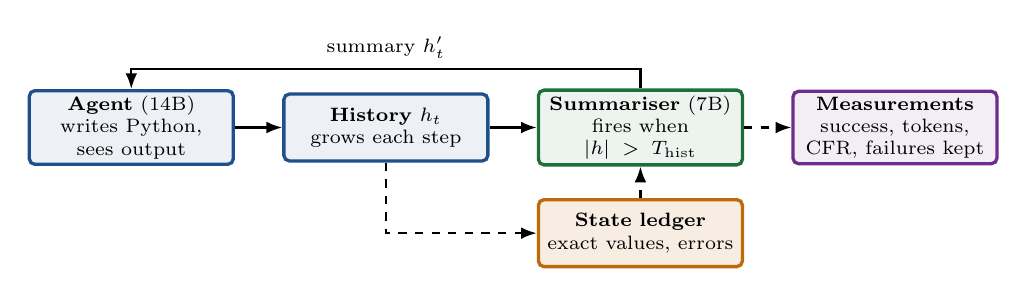
\begin{tikzpicture}[
  font=\scriptsize,
  bx/.style={draw, rounded corners=2pt, very thick, align=center,
    text width=2.45cm, minimum height=0.85cm, inner sep=2pt},
  arr/.style={-{Latex[length=2mm]}, line width=0.8pt},
  env/.style={bx, fill=envblue!8,  draw=envblue},
  cmp/.style={bx, fill=cmpgreen!8, draw=cmpgreen},
  ctl/.style={bx, fill=ctlorange!12, draw=ctlorange},
  met/.style={bx, fill=metviolet!8, draw=metviolet}]
\node[env] (ag) {\textbf{Agent} (14B)\\writes Python, sees output};
\node[env, right=6mm of ag] (h) {\textbf{History} $h_t$\\grows each step};
\node[cmp, right=6mm of h] (hc) {\textbf{Summariser} (7B)\\fires when $|h|>T_{\mathrm{hist}}$};
\node[met, right=6mm of hc] (m) {\textbf{Measurements}\\success, tokens,\\CFR, failures kept};
\node[ctl, below=4mm of hc] (led) {\textbf{State ledger}\\exact values, errors};
\draw[arr] (ag)--(h);
\draw[arr] (h)--(hc);
\draw[arr] (hc.north) -- ++(0,0.25) -| node[pos=0.25,above]{summary $h'_t$} (ag.north);
\draw[arr, dashed] (h.south) |- (led.west);
\draw[arr, dashed] (led.north) -- (hc.south);
\draw[arr, dashed] (hc)--(m);
\end{tikzpicture}
\end{center}
\vspace{-0.1cm}
\begin{columns}[T]
\begin{column}{0.24\textwidth}
\begin{block}{1. State ledger}
\scriptsize
Deterministic extractor (AST $+$ regex, no LLM) appends a verbatim block:
REPL variables, credentials, APIs called with literal args, non-existent APIs,
last 3 errors. Halves: \emph{values} / \emph{errors}.
\end{block}
\end{column}
\begin{column}{0.24\textwidth}
\begin{block}{2. Guideline edits}
\scriptsize
ACON's optimised D.7 $+$ ``include key info from errors or failed attempts''
(\emph{keep-failures}); v2 also drops ``tool/API log output'' from D.7's
deletion rule.
\end{block}
\end{column}
\begin{column}{0.24\textwidth}
\begin{block}{3. Controls}
\scriptsize
At the same threshold: the \textbf{unoptimised} guideline (D.5) and a
\textbf{14B summariser} --- separating guideline and summariser capacity
from compression frequency.
\end{block}
\end{column}
\begin{column}{0.24\textwidth}
\begin{block}{4. Instrumentation}
\scriptsize
Per-request prompt/completion tokens and latency for both models; CFR for
every compression call; keyword test: does the summary mention failures in its
input?
\end{block}
\end{column}
\end{columns}
\end{frame}

% ============================== 6-10. IMPLEMENTATION AND RESULTS
\section{Implementation and Results}
\begin{frame}{Implementation and Results (1/5): Setup and Protocol}
\centering
\scriptsize
\renewcommand{\arraystretch}{1.12}
\setlength{\tabcolsep}{4pt}
\begin{tabular}{p{0.13\textwidth}p{0.25\textwidth}p{0.54\textwidth}}
\toprule
\textbf{Item} & \textbf{ACON paper} & \textbf{This work}\\
\midrule
Agent       & gpt-4.1 & \texttt{qwen2.5:14b} (Q4\_K\_M), 16,384-token context\\
Compressor  & gpt-4.1 / distilled Qwen3-14B & \texttt{qwen2.5:7b}; \texttt{qwen2.5:14b} as a control\\
Guidelines  & optimised with o3 & paper's own optimised prompts copied verbatim (D.7 history, D.10 obs.); unoptimised D.5 as baseline\\
Thresholds  & $T_{\mathrm{hist}}=4096$, $T_{\mathrm{obs}}=1024$ & $T_{\mathrm{hist}}\in\{512,1024,2048,4096\}$, $T_{\mathrm{obs}}=256$\\
Splits      & train for optimisation & train 90 $+$ dev 57 for development; \textbf{test\_normal 168 held out}\\
\bottomrule
\end{tabular}

\vspace{0.15cm}
\begin{columns}[T]
\begin{column}{0.48\textwidth}
\begin{block}{Evaluation protocol}
\footnotesize
\begin{itemize}
  \item 2$\times$ RTX 2000 Ada (16\,GB), Ollama 0.20.0, identical weights;
        $\approx$2,900 task runs, temperature 0, $\le$30 steps
  \item Design choices on train/dev only; test used once per fixed config
  \item Paired stats: McNemar $+$wins$/-$losses, bootstrap 95\% CI
\end{itemize}
\end{block}
\end{column}
\begin{column}{0.48\textwidth}
\begin{block}{SAC reproduction and SAC\,$\times$\,ACON pilot}
\footnotesize
\begin{itemize}
  \item Released checkpoints within 0.1 F1: $15\times$ \textbf{54.98 / 39.25}
        (published 54.95 / 39.26)
  \item Failure-gated distillation: no effect ($-0.23$ ID F1) --- teacher
        worse on 90.5\% of examples
  \item Task-guided anchors $+$8.7 ID F1, but query-aware $\Rightarrow$ focus
        moved to ACON
\end{itemize}
\end{block}
\end{column}
\end{columns}
\end{frame}

\begin{frame}{Implementation and Results (2/5): RQ1 --- Combining Both Compressors}
\centering
\scriptsize
\renewcommand{\arraystretch}{1.15}
\setlength{\tabcolsep}{4.5pt}
\resizebox{0.92\textwidth}{!}{%
\begin{tabular}{lcccccc}
\toprule
\textbf{Arm} ($T_{\mathrm{hist}}{=}512$, $T_{\mathrm{obs}}{=}256$) & \textbf{Solved} &
\textbf{Rate (\%)} & \textbf{Steps} & \textbf{Peak tok.} & \textbf{Agent tok./task} &
\textbf{vs.\ none (McNemar)}\\
\midrule
No compression        & 100/147 & 68.0 & 18.0 & 8,256 & 104.5k & --\\
History               & 87/147  & 59.2 & 20.1 & 4,521 & 57.5k  & $+23/-36$, $p=0.12$\\
Observation           & 101/147 & 68.7 & 17.9 & 6,354 & 85.8k  & $+25/-24$, $p=1.0$\\
History + observation & 90/147  & 61.2 & 19.7 & \textbf{3,108} & \textbf{53.8k} & $+27/-37$, $p=0.26$\\
\bottomrule
\end{tabular}}

\vspace{0.15cm}
\begin{columns}[T]
\begin{column}{0.44\textwidth}
\centering
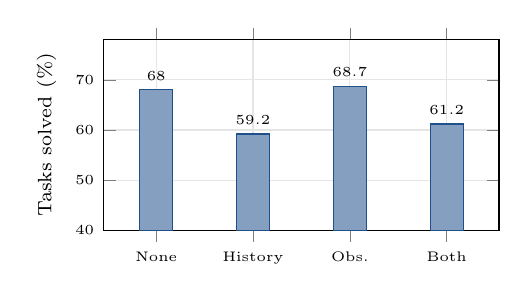
\begin{tikzpicture}
\begin{axis}[
  width=6.6cm, height=4.0cm,
  ybar, bar width=12pt,
  symbolic x coords={none,hist,obs,both},
  xtick=data,
  xticklabels={None,History,Obs.,Both},
  ylabel={Tasks solved (\%)}, ymin=40, ymax=78,
  nodes near coords, nodes near coords style={font=\tiny},
  tick label style={font=\tiny}, label style={font=\scriptsize},
  grid=major, grid style={gray!20}, enlarge x limits=0.18,
]
\addplot[fill=envblue!55, draw=envblue] coordinates {(none,68.0) (hist,59.2) (obs,68.7) (both,61.2)};
\end{axis}
\end{tikzpicture}
\end{column}
\begin{column}{0.54\textwidth}
\begin{block}{Result: ACON's penalty does not reproduce}
\footnotesize
\begin{itemize}
  \item Observation compression is neutral; history at 512 costs 8.8 points
  \item Combining costs \emph{less} than history alone:
        $I=\mathbf{+1.4}$ (95\% CI $[-10.2,+12.2]$) vs.\ ACON's $-9.5$
  \item With ACON's optimised guidelines on dev, $I$ is again positive
        ($+16.1$ at 512, $0.0$ at 4096)
  \item $\Rightarrow$ the mid-semester schedule-replay pipeline was
        \textbf{not needed}
\end{itemize}
\end{block}
\end{column}
\end{columns}
\end{frame}

\begin{frame}{Implementation and Results (3/5): RQ2 --- Threshold Sweep}
\begin{columns}[T]
\begin{column}{0.49\textwidth}
\centering
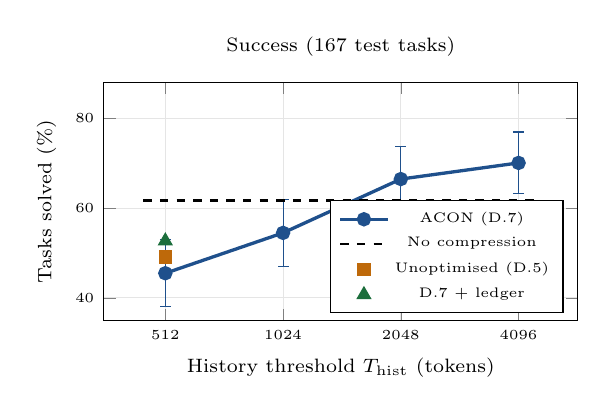
\begin{tikzpicture}
\begin{axis}[
  width=7.6cm, height=4.6cm,
  xmode=log, log basis x=2,
  xtick={512,1024,2048,4096}, xticklabels={512,1024,2048,4096},
  xlabel={History threshold $T_{\mathrm{hist}}$ (tokens)},
  ylabel={Tasks solved (\%)},
  ymin=35, ymax=88,
  grid=major, grid style={gray!20},
  legend style={font=\tiny, at={(0.97,0.03)}, anchor=south east},
  tick label style={font=\tiny}, label style={font=\scriptsize},
  title={\scriptsize Success (167 test tasks)},
]
\addplot[very thick, envblue, mark=*,
  error bars/.cd, y dir=both, y explicit]
  coordinates {(512,45.5) +- (0,7.5) (1024,54.5) +- (0,7.5) (2048,66.5) +- (0,7.2) (4096,70.1) +- (0,6.9)};
\addlegendentry{ACON (D.7)}
\addplot[thick, dashed, black] coordinates {(450,61.7) (4600,61.7)};
\addlegendentry{No compression}
\addplot[only marks, mark=square*, ctlorange, mark size=2.2pt] coordinates {(512,49.1)};
\addlegendentry{Unoptimised (D.5)}
\addplot[only marks, mark=triangle*, cmpgreen, mark size=2.8pt] coordinates {(512,52.7)};
\addlegendentry{D.7 + ledger}
\end{axis}
\end{tikzpicture}
\end{column}
\begin{column}{0.49\textwidth}
\centering
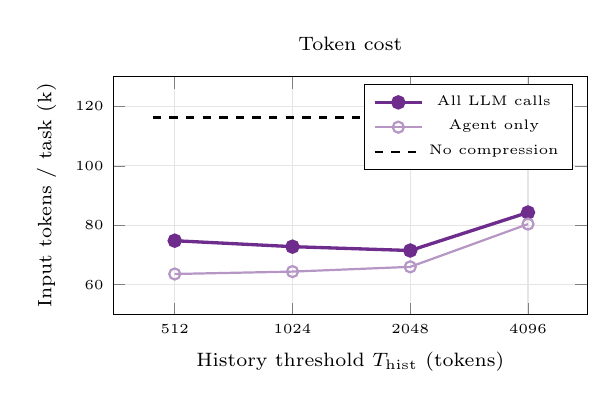
\begin{tikzpicture}
\begin{axis}[
  width=7.6cm, height=4.6cm,
  xmode=log, log basis x=2,
  xtick={512,1024,2048,4096}, xticklabels={512,1024,2048,4096},
  xlabel={History threshold $T_{\mathrm{hist}}$ (tokens)},
  ylabel={Input tokens / task (k)},
  ymin=50, ymax=130,
  grid=major, grid style={gray!20},
  legend style={font=\tiny, at={(0.97,0.97)}, anchor=north east},
  tick label style={font=\tiny}, label style={font=\scriptsize},
  title={\scriptsize Token cost},
]
\addplot[very thick, metviolet, mark=*] coordinates {(512,74.8) (1024,72.8) (2048,71.5) (4096,84.3)};
\addlegendentry{All LLM calls}
\addplot[thick, metviolet!50, mark=o] coordinates {(512,63.6) (1024,64.4) (2048,66.0) (4096,80.4)};
\addlegendentry{Agent only}
\addplot[thick, dashed, black] coordinates {(450,116.3) (4600,116.3)};
\addlegendentry{No compression}
\end{axis}
\end{tikzpicture}
\end{column}
\end{columns}

\vspace{0.1cm}
\footnotesize
\begin{itemize}
  \item \textbf{ACON works at its own threshold:} 70.1\% vs.\ 61.7\% uncompressed
        ($+8.4$, CI $[+0.0,+17.4]$), 31\% fewer agent tokens, less LLM time (181\,s vs.\ 199\,s)
  \item \textbf{Then it falls monotonically:} 70.1 $\to$ 66.5 $\to$ 54.5 $\to$ \textbf{45.5\%};
        4096 vs.\ 512: $+53/-12$, $p=2.8\times10^{-7}$; at 512, \textbf{16.2 points below} no compression
  \item \textbf{No token saving either:} total LLM input is lowest at 2048 (71.5k) and higher at 512 (74.8k)
\end{itemize}
\end{frame}

\begin{frame}{Implementation and Results (4/5): Held-Out Test --- All Arms}
\centering
\scriptsize
\renewcommand{\arraystretch}{1.12}
\setlength{\tabcolsep}{3pt}
\resizebox{\textwidth}{!}{%
\begin{tabular}{lcccccccc}
\toprule
\textbf{Arm (test, 167 tasks)} & \textbf{Solved} & \textbf{Rate (\%)} & \textbf{Steps} &
\textbf{Step cap hit} & \textbf{Peak tok.} & \textbf{Agent tok./task} & \textbf{All-LLM tok./task} &
\textbf{Compr./task}\\
\midrule
No compression                       & 103 & 61.7 & 18.8 & 64 & 8,806 & 116.3k & 116.3k & 0\\
\midrule
D.7, $T_{\mathrm{hist}}=4096$ (paper) & \textbf{117} & \textbf{70.1} & 18.3 & 50 & 6,584 & 80.4k & 84.3k & 0.7\\
D.7, $T_{\mathrm{hist}}=2048$         & 111 & 66.5 & 18.6 & 56 & 5,013 & 66.0k & \textbf{71.5k} & 1.9\\
D.7, $T_{\mathrm{hist}}=1024$         & 91  & 54.5 & 21.2 & 76 & 4,237 & 64.4k & 72.8k & 4.5\\
D.7, $T_{\mathrm{hist}}=512$          & 76  & 45.5 & 22.7 & 91 & 3,768 & 63.6k & 74.8k & 9.0\\
\midrule
\multicolumn{9}{l}{\emph{Controls and fixes at $T_{\mathrm{hist}}=512$}}\\
Unoptimised guideline (D.5)          & 82  & 49.1 & 21.6 & 85 & 4,096 & 62.2k & 72.7k & 8.9\\
D.7, 14B summariser                  & 78  & 46.7 & 22.4 & 89 & n/a   & n/a   & 75.0k & 9.4\\
D.7 + ledger, errors only            & 81  & 48.5 & 22.7 & 86 & 4,025 & 65.0k & 79.3k & 11.4\\
D.7 + full ledger                    & 88  & 52.7 & 21.7 & 79 & 4,173 & 67.1k & 89.0k & 15.6\\
\bottomrule
\end{tabular}}

\vspace{0.2cm}
\begin{columns}[T]
\begin{column}{0.48\textwidth}
\begin{block}{Why accuracy falls}
\footnotesize
\begin{itemize}
  \item 4096 $\to$ 512: history rewritten \textbf{13$\times$ as often}
        (0.7 $\to$ 9.0 per task)
  \item Agent loses track of progress: \textbf{54.5\%} of tasks hit the
        30-step cap vs.\ 29.9\%
\end{itemize}
\end{block}
\end{column}
\begin{column}{0.48\textwidth}
\begin{alertblock}{Not the guideline, size or value loss (RQ3)}
\footnotesize
\begin{itemize}
  \item D.5 $\approx$ D.7 ($p=0.50$); 14B summariser $\approx$ 7B ($p=0.89$)
  \item Full ledger $+$7.2 ($p=0.13$), errors-only $+$3.0 ($p=0.58$): not significant
\end{itemize}
\end{alertblock}
\end{column}
\end{columns}
\end{frame}

\begin{frame}{Implementation and Results (5/5): RQ3 --- The Dev Split Misled Us}
\begin{columns}[T]
\begin{column}{0.56\textwidth}
\centering
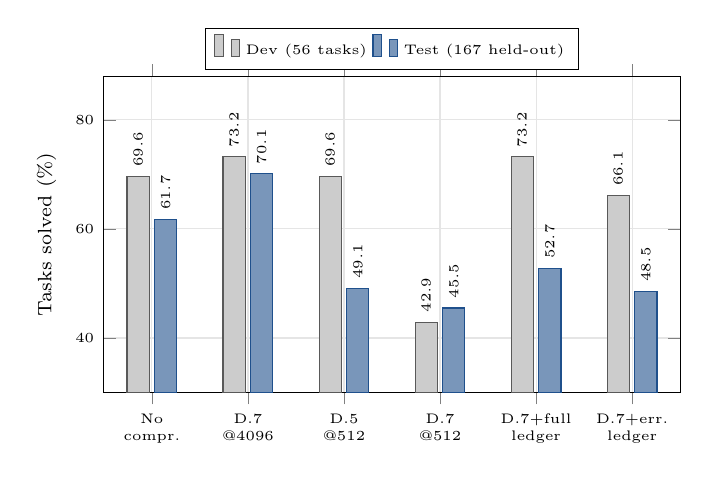
\begin{tikzpicture}
\begin{axis}[
  width=8.9cm, height=5.6cm,
  ybar, bar width=8pt,
  symbolic x coords={none,d74,d5s,d7s,full,err},
  xtick=data,
  xticklabels={{No\\compr.},{D.7\\@4096},{D.5\\@512},{D.7\\@512},{D.7+full\\ledger},{D.7+err.\\ledger}},
  xticklabel style={font=\tiny, align=center},
  ylabel={Tasks solved (\%)}, ymin=30, ymax=88,
  nodes near coords, nodes near coords style={font=\tiny, rotate=90, anchor=west},
  legend style={font=\tiny, at={(0.5,1.02)}, anchor=south, legend columns=2},
  tick label style={font=\tiny}, label style={font=\scriptsize},
  grid=major, grid style={gray!20}, enlarge x limits=0.1,
]
\addplot[fill=gray!40, draw=gray!70!black] coordinates {(none,69.6) (d74,73.2) (d5s,69.6) (d7s,42.9) (full,73.2) (err,66.1)};
\addlegendentry{Dev (56 tasks)}
\addplot[fill=envblue!60, draw=envblue] coordinates {(none,61.7) (d74,70.1) (d5s,49.1) (d7s,45.5) (full,52.7) (err,48.5)};
\addlegendentry{Test (167 held-out)}
\end{axis}
\end{tikzpicture}
\end{column}
\begin{column}{0.42\textwidth}
\begin{block}{On dev: a clear mechanism}
\scriptsize
\begin{itemize}
  \item D.7 says ``delete tool/API log output'': its summaries mention failures
        \textbf{32\%} of the time vs.\ 87\% for D.5
  \item Agents repeat failed attempts and call non-existent APIs (46\% vs.\ 36\% of steps)
  \item Every fix helped; full ledger \textbf{73.2\%} ($p=0.0015$). CFR did not
        predict success ($r=-0.08$)
\end{itemize}
\end{block}
\begin{alertblock}{On test: none of it held}
\scriptsize
\begin{itemize}
  \item D.5 collapses like D.7 despite mentioning failures 85\% vs.\ 26\%
  \item On 56 tasks one task $=$ 1.8 points; 10--15 point gaps were unstable
  \item What matters is the \textbf{number of rewrites}, not what the guideline keeps
\end{itemize}
\end{alertblock}
\end{column}
\end{columns}
\end{frame}

% ============================== 11. RESEARCH GAPS
\section{Research Gaps}
\begin{frame}{Research Gaps}
\begin{columns}[T]
\begin{column}{0.48\textwidth}
\begin{block}{Mid-semester gaps --- now settled}
\footnotesize
\begin{itemize}
  \item[(a)] \textbf{Latency.} At 4096 compression \emph{reduces} LLM time per
        task (181\,s vs.\ 199\,s); overhead appears only at 512 (255\,s)
  \item[(b)] \textbf{Confounded combined setting.} Penalty does not occur
        ($I=+1.4$, CI $[-10.2,+12.2]$) $\Rightarrow$ schedule replay not needed
  \item[(c)] \textbf{No intrinsic quality metric.} CFR implemented for every
        compression call, but does not predict success ($r=-0.08$)
\end{itemize}
\end{block}
\end{column}
\begin{column}{0.48\textwidth}
\begin{alertblock}{New gaps identified this semester}
\footnotesize
\begin{itemize}
  \item[(d)] \textbf{Benefit depends on compression frequency.} ACON reports
        one threshold; on held-out tasks success falls 70.1\% $\to$ 45.5\%,
        below no compression, with no token saving
  \item[(e)] \textbf{The guideline is not the cause.} At 512, optimised and
        unoptimised guidelines tie (45.5\% vs.\ 49.1\%, $p=0.50$) ---
        guideline optimisation does not protect against frequent compression
  \item[(f)] \textbf{Small dev splits mislead.} Three fixes chosen on 56 dev
        tasks reversed on 167 test tasks; guideline optimisation on small
        splits faces the same risk
\end{itemize}
\end{alertblock}
\end{column}
\end{columns}
\end{frame}

% ============================== 12. CONCLUSION AND FUTURE WORK
\section{Conclusion and Future Work}
\begin{frame}{Conclusion and Future Work}
\begin{columns}[T]
\begin{column}{0.49\textwidth}
\begin{block}{Conclusion}
\footnotesize
\begin{itemize}
  \item ACON reproduced with open-weight models: at its own threshold it
        \textbf{improves success and cuts tokens}
  \item Compressing more often \textbf{reverses} the benefit
        (70.1\% $\to$ 45.5\%) with no token saving
  \item Collapse persists under the unoptimised guideline, a 2$\times$ larger
        summariser and a deterministic ledger
  \item \textbf{Recommendation:} keep $T_{\mathrm{hist}}$ at 2048--4096 ---
        best accuracy (66.5--70.1\%) and lowest total cost (71.5--84.3k tok.)
\end{itemize}
\end{block}
\end{column}
\begin{column}{0.49\textwidth}
\begin{block}{Future work}
\footnotesize
\begin{itemize}
  \item \textbf{Complete the guideline $\times$ threshold curve:} D.5 at
        1024/2048/4096 and a repeat of D.7 at 512 (in progress)
  \item \textbf{Generalise:} second agent model family, second benchmark
  \item \textbf{Adaptive triggers:} compress at sub-task boundaries, not a
        fixed token count
  \item \textbf{Publication:} short paper reporting the dev-vs-test reversals
\end{itemize}
\end{block}
\begin{alertblock}{Limitations}
\footnotesize
One benchmark, one 4-bit model family; guidelines copied, not re-optimised;
one run per config (repeat differed on 1/56 tasks); failure mention is a keyword test.
\end{alertblock}
\end{column}
\end{columns}
\end{frame}

% ============================== 13. REFERENCES
\section*{References}
\setbeamertemplate{bibliography item}[text]
\begin{frame}{References}
\scriptsize
\begin{thebibliography}{9}
\bibitem{ACON} \textcolor{cmpgreen}{\textbf{$\bigstar$\,Used}} M. Kang, W.-N. Chen, D. Han, H. A. Inan, L. Wutschitz, Y. Chen,
R. Sim, and S. Rajmohan, ``ACON: Optimizing Context Compression for
Long-horizon LLM Agents,'' \emph{ICML}, PMLR 306, 2026.
\bibitem{SAC} \textcolor{cmpgreen}{\textbf{$\bigstar$\,Used}} X. Liu, R. Zhao, P. Huang, X. Liu, J. Xiao, C. Xiao, T. Xiao,
S. Gao, Z. Yu, and J. Zhu, ``Autoencoding-Free Context Compression for LLMs via
Contextual Semantic Anchors,'' \emph{ICLR}, 2026.
\bibitem{SWEPruner} Y. Wang, Y. Shi, M. Yang, R. Zhang, S. He, H. Lian,
Y. Chen, S. Ye, K. Cai, and X. Gu, ``SWE-Pruner: Self-Adaptive Context Pruning
for Coding Agents,'' arXiv:2601.16746, 2026.
\bibitem{LLMLingua} H. Jiang, Q. Wu, C.-Y. Lin, Y. Yang, and L. Qiu,
``LLMLingua: Compressing Prompts for Accelerated Inference of Large Language
Models,'' \emph{EMNLP}, pp.~13358--13376, 2023.
\bibitem{MEM1} Z. Zhou et al., ``MEM1: Learning to Synergize Memory and
Reasoning for Efficient Long-Horizon Agents,'' arXiv:2506.15841, 2025.
\bibitem{MemAgent} H. Yu et al., ``MemAgent: Reshaping Long-Context LLM with
Multi-Conv RL-based Memory Agent,'' \emph{ICLR}, 2026.
\bibitem{AppWorld} \textcolor{cmpgreen}{\textbf{$\bigstar$\,Used}} H. Trivedi et al., ``AppWorld: A Controllable World of Apps
and People for Benchmarking Interactive Coding Agents,'' \emph{ACL},
pp.~16022--16076, 2024.
\end{thebibliography}
\vspace{0.1cm}
{\scriptsize\textcolor{cmpgreen}{$\bigstar$\,\textbf{Used}} = used directly in our work: ACON is the base method (reproduced and stress-tested), SAC is reproduced and extended (SAC\,$\times$\,ACON pilot), AppWorld is our benchmark.}
\end{frame}

% ============================== 14. THANK YOU
{
\setbeamertemplate{footline}{}
\begin{frame}[plain]
\vspace{1.0cm}
\begin{center}
  \includegraphics[height=1.5cm]{"png college logo".png}

  \vspace{0.7cm}
  {\Huge\bfseries\color{envblue} Thank You}

  \vspace{0.5cm}
  \rule{0.45\textwidth}{0.8pt}

  \vspace{0.5cm}
  {\Large Questions?}

  \vspace{1.0cm}
  \footnotesize
  \begin{tabular}{r@{\hspace{0.8em}}l}
    \textbf{123CS0006} & Ayush Rahate\\
    \textbf{123CS0054} & Rohit Chauhan
  \end{tabular}

  \vspace{0.4cm}
  \footnotesize Supervisor: Dr.~N.~Srinivas Naik
\end{center}
\end{frame}
}

\end{document}
